% Copyright (c) 2019 Robert Ryszard Paciorek <rrp@opcode.eu.org>
% 
% MIT License
% 
% Permission is hereby granted, free of charge, to any person obtaining a copy
% of this software and associated documentation files (the "Software"), to deal
% in the Software without restriction, including without limitation the rights
% to use, copy, modify, merge, publish, distribute, sublicense, and/or sell
% copies of the Software, and to permit persons to whom the Software is
% furnished to do so, subject to the following conditions:
% 
% The above copyright notice and this permission notice shall be included in all
% copies or substantial portions of the Software.
% 
% THE SOFTWARE IS PROVIDED "AS IS", WITHOUT WARRANTY OF ANY KIND, EXPRESS OR
% IMPLIED, INCLUDING BUT NOT LIMITED TO THE WARRANTIES OF MERCHANTABILITY,
% FITNESS FOR A PARTICULAR PURPOSE AND NONINFRINGEMENT. IN NO EVENT SHALL THE
% AUTHORS OR COPYRIGHT HOLDERS BE LIABLE FOR ANY CLAIM, DAMAGES OR OTHER
% LIABILITY, WHETHER IN AN ACTION OF CONTRACT, TORT OR OTHERWISE, ARISING FROM,
% OUT OF OR IN CONNECTION WITH THE SOFTWARE OR THE USE OR OTHER DEALINGS IN THE
% SOFTWARE.

\ifdefined\inputOnlyContent\else
\documentclass{pdfBooklets}

\title{Laboratorium programistyczne:\\ Sumator i zastosowania automatów}
\author{%
	Projekt ,,Matematyka dla Ciekawych Świata'',\\
	Robert Ryszard Paciorek\\\normalsize\ttfamily <rrp@opcode.eu.org>
}
\date  {2019-05-09}

\makeatletter\hypersetup{
	pdftitle = {\@title}, pdfauthor = {\@author}
}\makeatother


\usepackage{tikz}
\usetikzlibrary{positioning} % for positionig nodes with `right = of X`
\usetikzlibrary{automata} % for initial and accepting nodes in tikzpicture graphs
\usetikzlibrary{arrows.meta, decorations.markings} % for arrows formating in tikzpicture
\usetikzlibrary{shapes} % for elipse nodes

\tikzset{
  arrowOuter/.style args={#1 colored by #2}{
    line width=#1, #2,
    decoration = {markings, mark=at position -0.01pt with \arrow{Kite[length=(#1),width=5*(#1)/2,inset=0,#2]}},
    preaction = {decorate}, % put arrow via decoration to prevent move due to shorten
    shorten >= {3*(#1)/4},  % use shorten to cut line inside arrow
  },
  arrowInner/.style args={#1 colored by #2 and scale by #3}{
    line width=#1-4*#3/3, #2,
    decoration = {markings, mark=at position -7*#3/8 with \arrow{Kite[length=(#1-3*#3/2),width=5*(#1-3*#3/2)/2,inset=0,#2]}},
    preaction = {decorate}, % put arrow via decoration to prevent move due to shorten
    shorten >= {3*(#1)/4 - #3/4},  % use shorten to cut line inside arrow
  },
  arrowDouble/.style args={#1 colored by #2}{
    double, line width=#1/6, double distance=2*#1/3, #2,
    decoration = {markings, mark=at position -0.01pt with \arrow{Kite[length=(#1),width=5*(#1)/2,inset=0,line width=11*#1/60,open,#2]}},
    preaction = {decorate}, % put arrow via decoration to prevent move due to shorten
    shorten >= {49*#1/60 - 0.015pt},  % use shorten to cut line inside arrow
    %postaction = {draw, line width=2*#1/3, green, shorten >= {3*(#1)/4}}
  },
  invisibleNode/.style={inner sep=0, outer sep = 0pt, minimum size=0},
}

\definecolor{xgreen}{rgb}{0.0,0.55,0.0}
\definecolor{xgray}{rgb}{0.45,0.45,0.45}

\begin{document}

\maketitle
\fi

%  BEGIN: Systemy liczbowe 01
\section{Systemy liczbowe}

Liczby mogą być zapisywane w różny sposób. Istnieją systemy addytywne (np. rzymski), w których istotna jest ilość powtórzeń danego elementu oraz systemy pozycyjne o różnych podstawach (np. system dziesiętny), w których istotne jest miejsce w którym znajduje się dany element.

W życiu codziennym najczęściej spotykamy się z zapisem dziesiętnym, funkcjonującym następująco: $5731 = 10^0 \cdot 1 + 10^1 \cdot 3 + 10^2 \cdot 7 + 10^3 \cdot 5$.

\subsection{System dwójkowy}

Ze względu na sposób budowy elektroniki cyfrowej i komputerów w informatyce dużo częściej spotykamy się z systemem dwójkowym (oraz systemami łatwo rozkładającymi się na dwójkowy, np. szesnastkowym).

Pojedynczą cyfrę systemu dwójkowego (przybierającą wartość 0 albo 1) określa się mianem \emph{bit}u, liczby reprezentowane są jako ciągi takich cyfr. Terminem \emph{bajt} określa się zazwyczaj ciąg o długości 8 bitów (ale w niektórych systemach ciąg o innej długości).

Podstawowym sposobem zapisy liczb całkowitych nie ujemnych w systemie dwójkowym jest \emph{naturalny kod binarny} (\emph{NKB}), w którym np. 4 bitowy ciąg {\tt a\textsubscript{3}a\textsubscript{2}a\textsubscript{1}a\textsubscript{0}} reprezentuje liczbę $2^0 \cdot a_0 + 2^1 \cdot a_1 + 2^2 \cdot a_2 + 2^3 \cdot a_3$. Zwróć uwagę na podobieństwo do systemu dziesiętnego.

Podstawowym sposobem zapisy liczb całkowitych (ze znakiem) jest \emph{kod uzupełnień do dwóch} (\emph{U2}) w którym n-bitowa liczba reprezentowana przez ciąg {\tt a\textsubscript{n-1}...a\textsubscript{3}a\textsubscript{2}a\textsubscript{1}a\textsubscript{0}} będzie miała wartość $2^0 \cdot a_0 + 2^1 \cdot a_1 + 2^2 \cdot a_2 + ... + 2^{n-2} \cdot a_{n-2} - 2^{n-1} \cdot a_{n-1}$. Jako że najstarszy bit wchodzi z ujemną wagą, jego ustawienie na 1 oznacza liczbę ujemną (ale nie jest to kod znaku). Warto zauważyć kompatybilność z NKB.

Liczby zapisywane w tych kodowaniach systemu dwójkowego oznacza się często przy pomocy prefiksu "0b" albo sufiksu "b" (w Pythonie możemy stosować jedynie  zapis z prefiksem), np. {\tt 0b101 = 101b} reprezentuje liczbę 5 w systemie dziesiętnym ($2^0 \cdot 1 + 2^1 \cdot 0 + 2^2 \cdot 1 = 5$).

%Oprócz podanych istnieje jeszcze kilka stosowanych sposobów zapisu liczb binarnych takich jak (dla liczb bez znaku): kod "1 z n", kod Graya, kod Johnsona, (dla liczb ze znakiem): kod znak-moduł, kod uzupełnień do jedności (U1). Odmiennym zagadnieniem jest kodowanie liczb zmiennoprzecinkowych. Nie będziemy ich jednak omawiać na tych zajęciach.
%  END: Systemy liczbowe 01

%  BEGIN: Sumator
\section{Sumator}

Cyfrowe układy elektroniczne (także te składające się na nasze komputery) każdą liczbę traktują jako ciąg logicznych jedynek i zer (wartości True i False).
Spróbujemy zasymulować takie działanie w Pythonie i zastanowić się nad tym jak można zrealizować dodawanie takich liczb.

Jeżeli znamy i pamiętamy jeszcze metodę dodawania ,,w słupku'' (,,pod kreską'') to wiemy, że dodawanie dwóch n cyfrowych liczb możemy potraktować jako ciąg n dodawań dwóch liczb jednocyfrowych z obsługą przeniesienia.
Podobnie można postąpić przy sumowaniu liczb binarnych. Potrzebujemy zatem elementu, który będzie sumował 3 wartości logiczne (dwie pochodzące z sumowanych liczb, jedna z przeniesienia z poprzedniego elementu)
i generował wynik sumy oraz wartość przeniesienia dla następnego elementu.

\begin{Zadanie}{}{}
Zastanów się w jaki sposób, korzystają z poznanych funkcji logicznych (and, or, xor, not) można obliczyć wartość sumy dwóch cyfr binarnych a i b oraz wartość przeniesienia.

\emph{Wskazówka: zapisz tablicę prawdy dla tej operacji}

\begin{teacherOnly}
Zapisując tablicę prawdy dla takiej operacji:

\begin{tabular}{c|c||c|c}
a & b  &  suma & przeniesienie\\
\hline
0 & 0  &  0 & 0\\
1 & 0  &  1 & 0\\
0 & 1  &  1 & 0\\
1 & 1  &  0 & 1\\
\end{tabular}

możemy zauważyć że suma to a XOR b, natomiast przeniesienie to a AND b.
\end{teacherOnly}
\end{Zadanie}

\begin{Zadanie}{}{}
Spróbuj rozszerzyć poprzednie rozwiązanie, tak aby uwzględniać w sumowaniu przeniesienie z poprzedniego elementu.

\emph{Wskazówka: rozszerz tablicę prawdy o jedną kolumnę wejściową}

\begin{teacherOnly}

\begin{tabular}{c|c|c||c|c}
p & a & b  &  suma & przeniesienie\\
\hline
0 & 0 & 0  &  0 & 0\\
0 & 1 & 0  &  1 & 0\\
0 & 0 & 1  &  1 & 0\\
0 & 1 & 1  &  0 & 1\\
%
1 & 0 & 0  &  1 & 0\\
1 & 1 & 0  &  0 & 1\\
1 & 0 & 1  &  0 & 1\\
1 & 1 & 1  &  1 & 1\\
\end{tabular}

\vspace{6pt} Teraz jest to trudniej zauważyć, ale:
\begin{itemize}
\item suma to (a XOR b) XOR p
\item przeniesienie to (a AND b) OR (p AND (a OR b)), co jest równoważne (a AND b) OR (p AND (a XOR b)),\\
      gdyż XOR od OR różni się tylko dla a == b == 1, a ten przypadek załatwia i tak OR z (a AND b)
\end{itemize}

Można też pokazać i omówić animację z Wikipedii: \url{https://commons.wikimedia.org/wiki/File:Fulladder.gif}
\end{teacherOnly}
\end{Zadanie}

\begin{teacherOnly}
\vspace{8pt}\noindent\strong{Napisać na tablicy wzory na sumator:}\\
s = (a XOR b) XOR p\\
p = (a AND b) OR (p AND (a XOR b))\\
\end{teacherOnly}

\begin{Zadanie}{}{zadanie_FullAdder}
Napisz funkcję realizującą sumator. Funkcja powinna przyjmować 3 argumenty logiczne (wartości dwóch bitów do zsumowania oraz wartość przeniesienia) i zwracać wartość sumy i przeniesienia do następnego elementu.

\emph{Wskazówka: zwracanie dwóch elementów z funkcji najprościej zrealizować poprzez zwracanie dwu elementowej listy.}
\end{Zadanie}

Liczba 6 posiada zapis binarny 0b110. Czyli jeżeli chcielibyśmy przedstawić ją w postaci listy wartości logicznych byłoby to [0, 1, 1]. Zwróć uwagę na zmianę kolejność bitów: wynika ona z tego że w zapisie list element o indeksie zero podajemy jako pierwszy a w zapisie binarnym liczby bit zerowy (wchodzący z wagą $2^0$) jest jako ostatni. Dzięki takiemu zapisaniu liczb możemy użyć naszego sumatora do dodania wielo-bitowych liczb.

\begin{Zadanie}{\domowe{3}}{zadanie_sumator_list}
Napisz funkcję wykorzystującą sumator stworzony w zadaniu \ref{zadanie_FullAdder} do obliczania sumy dwóch liczb reprezentowanych jako listy wartości logicznych.
Na przykład dla argumentów \Verb{[True, False, True]}, \Verb{[False, True, True]} (odpowiadających liczbom 5 i 6) wynikiem powinna być lista \Verb{[True, True, False, True]} (odpowiadająca liczbie 11).

Rozwiązanie powinno działać poprawnie dla liczb o dowolnej ilości bitów, także w przypadku gdy liczba bitów poszczególnych liczb jest różna.
Rozwiązania działające tylko dla liczb o równej lub ustalonej liczbie bitów mogą otrzymać maksymalnie 2pkt.

\emph{Wskazówka: dodawanie elementu na koniec listy możliwe jest z użyciem metody \Verb{append}, można też zedefiniować listę o zadanej ilości elementów np. \Verb{5 * [False]} i tylko modyfikować wybrane elementy.}
\end{Zadanie}
%  END: Sumator


\section{Automaty skończone}

Już najprostszy z poznanych typów automatów, czyli automat skończony, znajduje szerokie zastosowania praktyczne m.in. w informatyce i elektronice. Model automatu używany jest m.in. do opisu działania niektórych protokołów komunikacyjnych, czy też algorytmów postępowania, a także do opisu i realizacji elektronicznych układów logicznych.

\subsection{opisy algorytmów}
W zastosowaniach informatycznych najczęściej:
\begin{itemize}
\item przejścia związane są z reakcją na działania użytkownika lub klienta
\item wykonaniu przejścia do nowego stanu towarzyszy też wykonanie jakiejś akcji (np. wysłanie odpowiedzi do klienta, zapamiętanie jakiś dodatkowych informacji)
\item stan automatu związany jest z stanem wewnętrznym realizowanego algorytmu
\end{itemize}

\subsubsection{Typowe sposoby implementacji automatów}


Najbardziej klasycznym przykładem implementacji algorytmu w postaci automatu jest (zazwyczaj nieskończona) pętla w ramach której:

\noindent\begin{minipage}[t]{0.61\textwidth}
\begin{itemize}
\item wczytujemy kolejne porcje danych odpowiedzialne za wywoływanie kolejnych przejść pomiędzy stanami automatu,
\item z użyciem instrukcji warunkowej {\tt if / else} (lub nie występującej w Pythonie instrukcji wyboru {\tt switch / case}) w oparciu o aktualny stan automatu wybieramy stosowne postępowanie,
\item w wyniku wykonanych operacji ustalamy nowy stan automatu.
\end{itemize}
\end{minipage}\hfill\begin{minipage}[t]{0.35\textwidth}
\vspace{-8pt}
\begin{minted}{python}
while True:
    x = pobierzDane()
    if stan == "A":
        stan = dzialaniaA(x)
    elif  stan == "B":
        stan = dzialaniaB(x)
    ...
\end{minted}
\end{minipage}

\begin{Zadanie}{}{zadanie_konczace_ab}
Zaimplementuj automat sprawdzający czy podane słowo należy do języka nad alfabetem słów kończących się ciągiem \Verb{ab}:

\vspace{-0.5cm}\begin{center}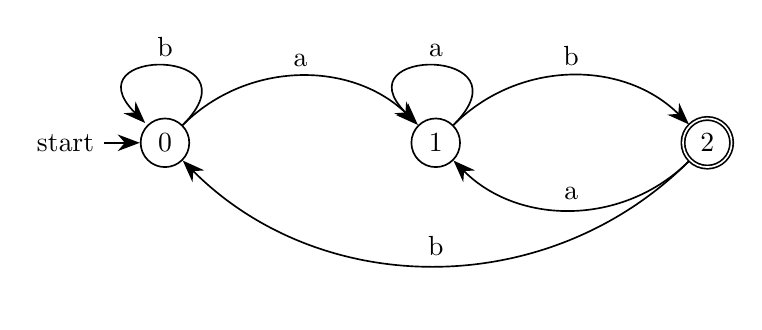
\begin{tikzpicture}[->, >={Stealth[length=8pt,width=6pt]}, node distance=2.8cm, semithick]
\node[circle, draw, initial] (0) {0};
\node[circle, draw] (A) [right = of 0] {1};
\node[circle, draw, accepting] (AB) [right = of A] {2};
\path (0)  edge [bend left=45] node[above] {a} (A);
\path (0)  edge [loop] node[above] {b} (0);
\path (A)  edge [bend left=45] node[above] {b} (AB);
\path (A)  edge [loop] node[above] {a} (A);
\path (AB) edge [bend left=45] node[above] {a} (A);
\path (AB) edge [bend left=45] node[above] {b} (0);
\end{tikzpicture}\end{center}\vspace{-0.5cm}

\emph{Wskazówka: zamiast \Verb{while True} możesz użyć pętli iterującej po literach słowa.}
\end{Zadanie}



\subsubsection{SMTP}

Oficjalna specyfikacja protokołu przesyłu poczty elektronicznej SMTP (Simple Mail Transfer Protocol) czyli \href{https://www.rfc-editor.org/info/rfc821}{RFC 821} nie definiuje tego protokołu bezpośrednio z użyciem automatu skończonego. Jednak możliwe jest opisanie go w taki sposób. Poniżej znajduje się graf automatu reprezentujący typową sesję protokołu SMTP (nie jest to pełen opis protokołu ani jego działania - pominięte zostały niektóre z obowiązkowych komend protokołu oraz zagadnienia weryfikacji).

\vspace{0.5cm}

\begin{adjustbox}{trim=2.95cm 0.7cm 0cm 0cm, clip=false, scale=.95}
\begin{tikzpicture} [ ->, >={Stealth[length=8pt,width=6pt]}, node distance=2.8cm, semithick, initial text={}, ]
	\tikzstyle{stan}=[ellipse, draw]
	\tikzstyle{klient}=[above, align=center, font=\footnotesize\tt\color{blue}]
	\tikzstyle{serwer}=[below, align=center, font=\footnotesize\tt\color{xgreen}]
	
	\node[stan, initial] (S0) {IDLE};
	\node[stan] (S2) [right = 2.5cm of S0] {C};
	\node[stan] (H)  [right = of S2] {HA};
	\node[stan] (MF) [right = 3.1cm of H]  {SA};
	\node[stan] (RT) [right = 3.1cm of MF] {RA};
	\node[stan] (DATA) [below = of RT] {DATA};
	
	\path
		(S2)
			edge[out=-90, in=-130, looseness=0.65]
				node[klient, pos=0.45] {QUIT}
				node[serwer, pos=0.45] {221 ... \textit{zamknięcie poł.}}
				(S0)
		(H)
			edge[out=-100, in=-130, looseness=0.9]
				node[klient] {QUIT}
				node[serwer] {221 ... \textit{zamknięcie poł.}}
				(S0)
		(MF)
			edge[out=-90, in=-130, looseness=1]
				node[klient] {QUIT}
				node[serwer] {221 ... \textit{zamknięcie poł.}}
				(S0)
		(RT)
			edge[out=-110, in=-130, looseness=1]
				node[klient] {QUIT}
				node[serwer] {221 ... \textit{zamknięcie poł.}}
				(S0)
		;
	\path
		(S0)
			edge
				node[klient] {\itshape nawiązanie\\\itshape połączenia}
				node[serwer] {220 ...}
				(S2)
		(S2)
			edge
				node[klient] {HELLO ...}
				node[serwer] {250 ...}
				(H)
		(H)
			edge[loop, out=30, in=150, looseness=7]
				node[klient] {...}
				node[serwer] {500 ...}
				(H)
			edge[loop, out=30, in=150, looseness=16]
				node[klient] {RCPT TO: ... \\ DATA}
				node[serwer] {503 ...}
				(H)
			edge
				node[klient] {MAIL FROM: ...}
				node[serwer] {250 ...}
				(MF)
			edge[out=-110, in=-160, looseness=11]
				node[klient,sloped] {RSET}
				node[serwer,sloped] {250 ...}
				(H)
		(MF)
			edge[loop, out=30, in=150, looseness=7]
				node[klient] {...}
				node[serwer] {500 ...}
				(MF)
			edge[loop, out=30, in=150, looseness=16]
				node[klient] {DATA}
				node[serwer] {503 ...}
				(MF)
			edge
				node[klient] {RCPT TO: ...}
				node[serwer] {250 ...}
				(RT)
			edge[out=-110, in=-70, looseness=0.7]
				node[klient] {RSET}
				node[serwer] {250 ...}
				(H)
		(RT)
			edge[loop, out=30, in=150, looseness=7]
				node[klient] {...}
				node[serwer] {500 ...}
				(RT)
			edge[loop, out=30, in=150, looseness=16]
				node[klient] {RCPT TO: ...}
				node[serwer] {250 ...}
				(RT)
			edge[out=-40, in=90]
				node[klient,sloped] {DATA ...}
				node[serwer,sloped] {250 ...}
				(DATA)
			edge[out=-110, in=-70]
				node[klient] {RSET}
				node[serwer] {250 ...}
				(H)
		(DATA)
			edge[loop, out=-20, in=-90, looseness=3]
				node[klient] {...}
				(DATA)
			edge[out=-150, in=-90]
				node[klient, pos=0.25] {\itshape pojedyncza\\\itshape kropka w linii}
				node[serwer, pos=0.25] {250 ...}
				(H)
	;
\end{tikzpicture}
\end{adjustbox}

\noindent
Poszczególne stany oznaczają:
\begin{itemize}
\item IDLE -- oczekiwanie na połączenie
\item C -- nawiązane połączenie w warstwie niższej (TCP)
\item HA -- otrzymano i zapamiętano informację o adresie klienta przekazanym w HELO (jest to nazwa hosta lub nazwa domenowa, ale nie adres poczty)
\item SA -- otrzymano i zapamiętano informację o adresie e-mail nadawcy
\item RA -- otrzymano i zapamiętano informację o adresach e-mail odbiorców (kolejne wejścia do tego stanu powodują dodanie kolejnego odbiorcy do listy)
\item DATA -- odbieranie treści maila (zakończenie przy pomocy linii złożonej wyłącznie z kropki, skutkuje zakolejkowaniem listu do wysyłki lub jego wysłaniem)
\end{itemize}

\noindent
Powyżej strzałek reprezentujących przejścia pomiędzy stanami (kolor niebieski) podane zostały działania i polecenia wysyłane przez klienta wywołujące dane przejście, zaś poniżej (kolor zielony) podane zostały odpowiedzi serwera.
W miejscu {\tt ...} występuje tekst stanowiący dane (np. adres nadawcy lub odbiorcy), komunikat związany z podanym kodem odpowiedzi lub dowolną, inną od wymienionych komendę.
Zapis przykładowej sesji protokołu SMTP opisywanej powyższym automatem:

{\vspace{0.3cm}\noindent\tt
   \hspace{1cm}\color{xgreen}220 dragon.icm.edu.pl ESMTP Exim 4.89 Fri, 26 Apr 2019 13:14:42 +0000
\\ \hspace{1cm}\color{blue}HELO test.example.com
\\ \hspace{1cm}\color{xgreen}250 dragon.icm.edu.pl Hello test.example.com [2001:6a0:0:21::60:13]
\\ \hspace{1cm}\color{blue}MAIL FROM: rrp@dragon.icm.edu.pl
\\ \hspace{1cm}\color{xgreen}250 OK
\\ \hspace{1cm}\color{blue}RCPT TO: rrp@dragon.icm.edu.pl
\\ \hspace{1cm}\color{xgreen}250 Accepted
\\ \hspace{1cm}\color{blue}DATA
\\ \hspace{1cm}\color{xgreen}354 Enter message, ending with "." on a line by itself
\\ \hspace{1cm}\color{blue}to jest e-mail, ale bez standardowych naglowkow ...
\\ \hspace{1cm}\color{blue}wiec bedzie dziwnie wygladal w programie klienckim ...
\\ \hspace{1cm}\color{blue}.
\\ \hspace{1cm}\color{xgreen}250 OK id=1hK0hn-0008FU-OV
\\ \hspace{1cm}\color{blue}QUIT
\\ \hspace{1cm}\color{xgreen}221 dragon.icm.edu.pl closing connection
\color{black}\vspace{0.3cm}}

\begin{Zadanie}{\domowe{3}}{zadanie_smtp}
\teacher{\strong{Uwaga:} Pomimo że zadanie sugeruję dać jako domowe to na zajęciach warto krótko omówić działanie tego automatu. }
Napisz symulator serwera SMTP w postaci wyżej przedstawionego automatu. Program powinien przyjmować kolejne komendy od użytkownika i stosownie na nie reagować.

\vspace{0.3cm}
\emph{Wskazówka: do wczytywania kolejnych linii w ramach pętli głównej automatu możesz użyć: \python{linia = sys.stdin.readline().rstrip()}.
                 Wymaga to wcześniejszego zaimportowania moduły sys poprzez: \python{import sys}.\student{\\}
                 Dzięki użyciu metody \python{rstrip()} wczytana linia nie będzie zawierała kończącego ją znaku nowej linii (ani innych białych znaków na końcu).
}
\end{Zadanie}

\subsection{elektronika – układy logiczne}

\subsubsection{opis automatu przy pomocy tablicy prawdy}

Jak pamiętamy z zajęć o sumatorze elektronicy lubią opisywać układy cyfrowe z użyciem tablic prawdy. W taki sposób można opisać także dowolny automat skończony.
W tym celu numerujemy (binarnie) stany automatu oraz pobudzenia wywołujące przejścia pomiędzy stanami (elementy alfabetu), numery te będziemy nazywać wektorami stanu i wektorami wejść.
Następnie tworzymy tablicę prawdy postaci:

\begin{center}\begin{tabular}{c|c|c|c|c|c|c|c||c|c|c|c}
$S_l$ & ... & $S_1$ & $S_0$   &   $I_k$ & ... & $I_1$ & $I_0$   &    $N_l$ & ... & $N_1$ & $N_0$\\
\hline
& & &   &   & & &   &   & & &
\end{tabular}\end{center}

\noindent
gdzie $S_l ... S_1 S_0$ to wektor stanu (czyli $l$ bitowy numer stanu), $I_k ... I_1 I_0$ to wektor wejść (czyli $l$ bitowy numer pobudzenia wywołującego zmianę stanu), a $N_l ... N_1 N_0$ to $l$ bitowy numer stanu do którego ma przejść automat znajdujący się w stanie określonym w kolumnach $S_l ... S_1 S_0$, pod wpływem pobudzenia podanego w kolumnach $I_k ... I_1 I_0$.
Wadą takiego opisu jest bardzo szybko rosnąca liczba wierszy w tabeli. Wynosi ona $2^{l+k}$, czyli np. dla 3 stanowego automatu z 2 bitowym wejściem jest ich już 32.

\subsubsection{realizacja pamięciowa}

Opis taki natomiast umożliwia bardzo prostą implementację w postaci „\emph{pamięciowej}”. Używając $l+k$ komórek pamięci, adresowanych ciągiem bitowym $S_l ... S_1 S_0 I_k ... I_1 I_0$, możemy w każdej z nich przechowywać po prostu numer następnego stanu (w związku z tym muszą to być co najmniej $l$ bitowe komórki pamięci). Ideę takiej realizacji automatu przedstawia poniższy schemat:

\begin{center}\begin{tikzpicture}[ ->, >={Stealth[length=8pt,width=6pt]}, semithick ]
	\node[draw, minimum height=6em, minimum width=10em,
		label={[label distance=-.7cm, text depth=3.5ex, rotate=90]right:DANE},
		label={[label distance=-.9cm, text depth=3.5ex, rotate=-90]left:ADRES}
		] (M) {PAMIĘĆ};
	
	\node[invisibleNode, above right = 2.2em and 2em of M] (rt) {};
	\node[invisibleNode, above left = 2.2em and 2em of M] (lt) {};
	\draw (M.0) -| (rt) -- node[below] {$S_l ... S_1 S_0 \quad \leftarrow \quad N_l ... N_1 N_0$} (lt) |- (M.165);
	%\draw (lt) edge[draw, red, ->, to path={|- (\tikztotarget)}] (M.165);
	
	\node[invisibleNode, left = 5em of M.195] (de) {};
	\draw (de) --node[below] {$I_k ... I_1 I_0$} (M.195);
\end{tikzpicture}\end{center}

\begin{ProTip}{Ciekawostka {\Symbola 🤔}}
Pamięć o $n$ bitowym rozmiarze pojedynczej komórki (i szyny danych) oraz o $m$ bitowej przestrzeni adresowej (i nie mniejszej szynie adresowej) stanowi bardzo prostą realizację bramki logicznej mogącej realizować dowolną funkcję logiczną. Dodatkowo funkcja ta może być programowo zmieniana. Własność ta jest powszechnie wykorzystywana w współczesnej elektronice i leży u podstaw działania układów o programowalnej strukturze, takich jak FPGA.
\end{ProTip}

\begin{Zadanie}{\domowe{2}}{zadanie_pamiec_8kB}
Czy pamięć o wielkości 8kB, złożona z komórek o wielkości 8bitów (i używająca takiej szerokości szyny danych), posiadająca 16 bitową szynę adresową\footnote{
	W przypadku gdy szyna adresowa udostępnia większą przestrzeń adresową niż rozmiar pamięci, najstarsze bity adresu są ignorowane.
	Oznacza to że w przypadku tej pamięci odwołanie do adresu $8{\rm k} + x$ (dokładnie $8*1024+x$), jest odwołaniem do adresu $x$.
} umożliwia realizację (w przedstawiony powyżej sposób) automatu o 8 stanach i 4 bitowym wejściu? Odpowiedź krótko uzasadnij.
\end{Zadanie}

\subsubsection{realizacja w postaci funkcji logicznej}

Jak wiemy (z zajęć o sumatorze) opis układu przy pomocy tablicy prawdy pozwala na jego realizację z użyciem standardowych funkcji logicznych (bramek and, or, not, xor). W ten sposób możemy także realizować automaty. Analogicznie jak na powyższym schemacie realizacji \emph{pamięciowej} będzie musiało wystąpić podanie sygnału z wyjścia bramek na ich wejście (sprzężenie zwrotne).

Realizacja taka jest bardziej oszczędna pod względem zasobów od realizacji \emph{pamięciowej}, jednak bardziej wymagająca na etapie projektowania – trzeba dokonać konwersji tablicy prawdy na funkcje logiczne. Konwersji takiej dokonujemy niezależnie dla każdego bitu nowego wektora stanu ($N_l ... N_1 N_0$), czyli musimy skonwertować $l$ tablic prawdy na $l$ funkcji logicznych, każda w ogólności\footnote{część argumentów może okazać się nieistotna dla obliczania danego $N_x$ – nie wpływać na jego wartość} o $l+k$ argumentach.

\begin{Zadanie}{}{automat_rs}
Przyjrzyj się poniższemu automatowi (y=x oznacza "gdy y ma wartość x", ? – dowolna wartość).
\begin{center}
\begin{adjustbox}{stack=cc}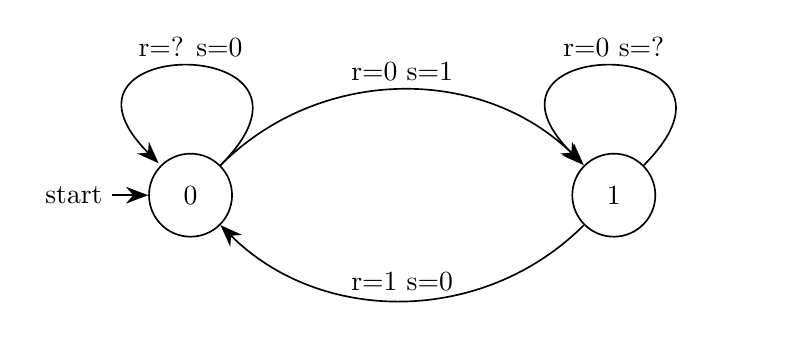
\begin{tikzpicture}[->, >={Stealth[length=8pt,width=6pt]}, node distance=4.3cm, semithick]
\node[circle, minimum size=3em, draw, initial] (0) {0};
\node[circle, minimum size=3em, draw] (1) [right = of 0] {1};
\path (0)  edge [bend left=45] node[above] {r=0 s=1} (1);
\path (1)  edge [bend left=45] node[above] {r=1 s=0} (0);

\path (0)  edge [loop] node[above] {r=? s=0} (0);
\path (1)  edge [loop] node[above] {r=0 s=?} (1);
\end{tikzpicture}\end{adjustbox}
\begin{tabular}{>{\centering}m{1.1cm}|>{\centering}m{1.1cm}|>{\centering}m{1.1cm}||c}
Stan & r & s & Nowy Stan\\
\hline
0 & 0 & 0 & 0\\
0 & 1 & 0 & 0\\
0 & 0 & 1 & 1\\
%0 & 1 & 1 & ?\\
1 & 0 & 0 & 1\\
1 & 1 & 0 & 0\\
1 & 0 & 1 & 1\\
%1 & 1 & 1 & ?
\end{tabular}
\end{center}

\begin{enumerate}
\item Czy zauważyłeś coś nietypowego?
	\teacher{
		Opis automatu jest niekompletny, nie określa działania w przypadku r=1 s=1.
		Taką sytuację traktujemy jako zabronioną i nie interesuje nas ona.
		Pozwala to na większą swobodę w konstrukcji automatu i łatwiejsze odnalezienie wyrażenia go opisującego.
	}
\item Spróbuj znaleźć wyrażenie logiczne realizujące ten automat.
	\teacher {
		Patrząc po wierszach dla których „Nowy Stan” ma wartość 1 uzyskujemy: \python{s or (Stan and not r)}.
	}
\item Zaimplementuj funkcję realizującą ten automat i użyj je do wypisania tablicy prawdy, celem weryfikacji poprawności działania.
\end{enumerate}

\begin{teacherOnly}
\begin{CodeFrame}[python]{0.65\textwidth}
def rs(s, r, q):
	return s or (q and not r)

for q in [0,1]:
  for s in [0,1]:
    for r in [0,1]:
      print(q, r, s, int(rs(s,r,q)))
\end{CodeFrame}
\begin{CodeFrame}[text][escapeinside=@@]{auto}
0 0 0 0
0 1 0 0
0 0 1 1
@\textcolor{xgray}{0 1 1 1}@
1 0 0 1
1 1 0 0
1 0 1 1
@\textcolor{xgray}{1 1 1 1}@
\end{CodeFrame}
\end{teacherOnly}

\begin{teacherOnly}
%\fontspec{lmroman12-regular}[Color=teacherColor]
\textcolor{\FSTop{colors}}{}\color{\FSTop{colors}}
Klasyczna realizacja w elektronice zatrzasku RS (z niezanegowanymi wejściami) składa się z dwóch bramek nor (not or):

\begin{center}
\includegraphics[width=0.45\textwidth]{img/elektronika/RS}
\end{center}

Ze względu na skomplikowane sprzężenie zwrotne, wymaga ona dwukrotnego przetworzenia stanu automatu i daje inne wyniki dla zabronionej sytuacji r=1 s=1:

\begin{CodeFrame}[python][]{0.65\textwidth}
def rs2(s, r, q, nq):
	return [not (r or nq), not (s or q)]

def rs(s, r, q):
	q, nq = rs2(s, r, q, not q)
	q, nq = rs2(s, r, q, nq)
	return q

for q in [0,1]:
  for s in [0,1]:
    for r in [0,1]:
      print(q, r, s, int(rs(s,r,q)))
\end{CodeFrame}
\begin{CodeFrame}[text][escapeinside=@@]{auto}
0 0 0 0
0 1 0 0
0 0 1 1
@\textcolor{xgray}{0 1 1 0}@
1 0 0 1
1 1 0 0
1 0 1 1
@\textcolor{xgray}{1 1 1 0}@
\end{CodeFrame}
\end{teacherOnly}
\end{Zadanie}

\subsubsection{asynchroniczne i synchroniczne}

Omówione do tej pory automaty charakteryzowały się brakiem jakiegokolwiek mechanizmu ustalania kiedy powinny odczytać stan wektora wejściowego i wykonać związane z nim przejścia.
Układy tego typu (które reagują na zmiany wejścia zachodzące w dowolnym momencie) nazywamy asynchronicznymi.

Niestety taka prosta realizacja napotyka kilka problemów:
\begin{itemize}
\item Automat nie uzyskuje żadnej informacji o tym, iż wektor wejściowy jest nowy (podana została nowa litera analizowanego słowa).
      W efekcie, jeżeli litera $v$ odpowiada za przejścia z A do B i z B do C, to automat na skutek podania jej na wejście może przeskoczyć z A do C zanim zostanie podana inna litera.
      Aby tego uniknąć każdy wektor wejściowy powodujący wejście do danego stanu powinien powodować pozostawanie w nim.
\item Zmiana kilku bitów wektora wejściowego praktycznie nigdy nie będzie równoczesna.
      W efekcie, jeżeli np. jesteśmy w stanie A (z którego możemy przejść pod wpływem $01$ do B, $10$ do C, $11$ do D) i następuje zmiana wektora wejściowego z $00$ na $11$ nie możemy przewidzieć do którego stanu przejdziemy (B, C czy może D).
      Aby uniknąć negatywnych skutków takiego działania automat taki powinien ze stanów B i C przechodzić do D pod wpływem wektora $11$.
\end{itemize}

\begin{ProTip}{Ciekawostka {\Symbola 🤔}}
Mianem układów asynchronicznych określane mogą być nie tylko automaty, ale też inne układy elektroniczne.
Nie wszystkie z omawianych problemów dotyczą wszystkich układów asynchronicznych.
Duża część tych problemów związana jest z faktem sprzężenia zwrotnego, z którym mamy do czynienia w konstrukcji automatu.
\end{ProTip}

Pomimo tych utrudnień w konstrukcji automaty asynchroniczne są spotykane w praktyce (zauważ, że wcześniej także skonstruowaliśmy poprawny automat asynchroniczny – przerzutnik RS).
Jednak ze względu na te problemy dużo częściej stosowane są automaty synchroniczne.

W automatach synchronicznych występuje dodatkowy sygnał zegarowy, służący do synchronizacji odczytu wejść i wykonywania przejść.
Można powiedzieć, że informuje on o tym, iż na wejściu przygotowana została kolejna litera analizowanego słowa i można wykonać związaną z nią zmianę stanu automatu.

\begin{ProTip}{Ciekawostka {\Symbola 🤔}}
W naturalny sposób prowadzi to do stosowania w realizacji automatów synchronicznych, jako komórek pamiętających poszczególne bity wektora stanu przerzutników typu D.
Przerzutniki te zapamiętują podawaną na nie informację w momencie narastającego bądź opadającego zbocza zegara i przechowują ją (oraz wystawiają na swoim wyjściu) do nadejścia kolejnego zbocza.
Ze względu na sposób działania pamięci, implementacje automatów oparte na niej na ogół w naturalny sposób są automatami synchronicznymi – funkcję zegara pełnią sygnały sterujące wykonaniem operacji odczytu.
\end{ProTip}

Zwróć uwagę, iż nasze implementacje automatów w Pythonie są dużo bliższe automatom synchronicznym niż asynachronicznym – nie mamy typowego okresowego sygnału zegarowego, ale jego funcję pełni zatwierdzenie wprowadzonych danych przy pomocy znaku nowej linii w \python{readline()}, bądź jawne wywołanie funkcji.


\subsubsection{automaty Moore'a i Mealy'ego}

W praktycznych zastosowaniach chcemy aby działanie układu elektronicznego realizującego dany automat objawiało się nie tylko zmianą stanów wewnętrznych automatu, ale przede wszystkim zmianą stanów jakiś wyjść.
Można zostać to zrealizowane na jeden z dwóch sposobów:
\begin{itemize}
\item Możemy ściśle powiązać stan wyjścia z stanem w którym się znajduje automat.
      W tym celu ustalamy funkcję logiczną przekształcającą wektor stanu na stan wyjść z nim związany (wektor wyjściowy).
      Ten typ automatu określamy mianem automatu Moore'a.
      W niektórych przypadkach możliwe jest takie zakodowanie automatu w taki sposób aby wektor stanu lub jego fragment stanowił bezpośrednio wektor wyjściowy (lub jego fragment).
      Jeżeli automat realizujemy w postaci \emph{pamięciowej} to wektor wyjściowy może być przechowywany w tych samych komórkach pamięci co wektor stanu.
\item Alternatywnie przy ustalaniu wartości wyjść oprócz bieżącego stanu automatu możemy także uwzględniać wartość wejść (pobudzenia, które spowodowało ostatnie przejście).
      Ten typ automatu określamy mianem automatu Mealy'ego.
      Często pozwala on na zmniejszenie ilości stanów automatu, kosztem bardziej rozbudowanej logiki wyjściowej.
\end{itemize}

\begin{Zadanie}[breakable]{}{zadanie_konczace_ab_pamieciowy}
Przypomnij sobie automat akceptujący słowa kończące się na ab z zadania \ref{zadanie_konczace_ab}.
Dodaj do tego automatu jedno bitowe wyjście informujące o tym że aktualnie wprowadzone słowo zostało zaakceptowane.
Możesz w tym celu wybrać rozwiązanie automatu Moore'a albo Mealy'ego. Wybór krótko uzasadnij.
Zapisz tablicę prawdy dla tego automatu i zasymuluj jego działanie w postaci pamięciowej.

\emph{Wskazówka: do zasymulowania pamięci możesz użyć słownika w którym kluczami są stałe listy\footnote{
	Stałą listę (nazywaną \emph{krotką}) zapisujemy używając nawiasów okrągłych zamiast kwadratowych, np. \Verb{(1, 2, 3)}. Możemy konwertować zwykłe listy na krotki przy pomocy \Verb{tuple()} i krotki na listy przy pomocy \Verb{list()}
} reprezentujące wektor stanu i wektor wejściowy, a wartościami reprezentują nowy wektor stanu.}
\end{Zadanie}

\begin{Zadanie}[breakable]{\domowe{1}}{zadanie_rs_pamieciowy}
Zaimplementuj automat z zadania \ref{automat_rs} w postaci pamięciowej, jako automat z jednobitowym wyjściem. Możesz w tym celu wybrać rozwiązanie automatu Moore'a albo Mealy'ego. Wybór krótko uzasadnij.
\end{Zadanie}


\subsubsection{realizacja w postaci układu mikro-programowalnego {\Symbola 🤔}}

Jeszcze innym podejściem do realizacji automatu w oparciu o pamięć jest układ mikro-programowalny. Jego działanie opiera się na przechowywaniu w pamięci instrukcji złożonych z pól: adresowych, kontrolnych, sterujących i operacyjnych.
W oparciu o aktualne dane wejściowe (z \emph{układu operacyjnego}) i aktualny stan (czyli wartość tych pól) wystawiane są dane wyjściowe (do \emph{układu operacyjnego}) oraz podejmowana jest decyzja o wyborze stanu następnego.
Poniżej znajduje się przykładowy schemat działania układu mikro-programowalnego.

\begin{center}\begin{adjustbox}{scale=.95}\begin{tikzpicture}[semithick, node distance=0.9cm]
	\tikzstyle{hor}=[rectangle, draw, minimum height=2.5em, minimum width=9em]
	\tikzstyle{vert}=[rectangle, draw, minimum height=2.5em, minimum width=9em, rotate=90]
	\tikzstyle{memory}=[rectangle, draw, minimum height=2.5em, anchor=north west, minimum width=24em, outer sep = 0pt]
	\tikzstyle{subMem}=[rectangle, draw, minimum height=1.7em, anchor=north west, minimum width=6em, outer sep = 0pt]
	\tikzstyle{da1}=[arrowDouble=8pt colored by black, rounded corners=5pt]
	\tikzstyle{da2}=[arrowInner=8pt colored by white and scale by 2pt, rounded corners=5pt]
	\tikzstyle{sa}=[draw, ->, >={Stealth[length=8pt,width=6pt]}]
	\tikzstyle{ssa}=[arrowOuter=7pt colored by xgray, rounded corners=5pt]
	
	\node[hor] (SUM)                      {\LARGE$\Sigma$};
	\node[hor, text depth=2.2ex] (MUX1)  [below = of SUM]   {MUX1};
		\draw[-] (MUX1.north west) -- (MUX1.-90); \draw[-] (MUX1.north east) -- (MUX1.-90);
	\node[hor] (COUNT) [below = of MUX1]  {Licznik};
	\node[memory] (MEM)   [below = of COUNT] {Pamięć};
		\node[subMem] (MEM_A) [] at (MEM.south west)   {adresowe};
		\node[subMem] (MEM_K) [] at (MEM_A.north east) {kontrolne};
		\node[subMem] (MEM_S) [] at (MEM_K.north east) {sterujące};
		\node[subMem] (MEM_O) [] at (MEM_S.north east) {operacyjne};
	
	\node[vert, text depth=2.2ex] (MUX2)  [below = 1.3cm of MEM_K, anchor=east]   {MUX2};
		\draw[-] (MUX2.north west) -- (MUX2.-90); \draw[-] (MUX2.north east) -- (MUX2.-90);
	\node[rectangle, draw, align=left, minimum height=7em, minimum width=6em] (DMI)  [above right = 0.7cm and 2.8cm of MUX2.south, anchor=west]   {Dekoder\\Mikro\\Instrukcji};
	
	% address sum-mem path
	\draw[da1] (SUM) -- (MUX1.90);
	\draw[da1] (MUX1) --  (COUNT.90);
	\draw[da1] (COUNT) -- (MEM.90);
	
	% address count-sum path
	\node[invisibleNode, above = 1.2em of MEM] (addr1) {};
	\node[invisibleNode, above right = 1.2em and 2.0em of MUX1] (addr2) {};
	\node[invisibleNode, above right = 1.2em and 0.0em of SUM] (addr3) {};
	\draw[da1] (addr1) -| (addr2) |- (addr3) -| (SUM.30);
	\draw[da1] (addr2) -| (MUX1.30);
	
	% filling fix
	\draw[da2] (addr1) -| (addr2) |- (addr3) -| (SUM.30);
	\draw[da2] (addr2) -| (MUX1.30);
	\draw[da2] (COUNT) -- (MEM.90);
	\draw[da2] (MUX1) --  (COUNT.90);
	\draw[da2] (SUM) -- (MUX1.90);
	
	% address mem-sum path
	\node[invisibleNode, below left = 1.2em and 0.0em of MEM_A] (addr5) {};
	\node[invisibleNode, above left = 1.2em and 2.0em of MEM_A] (addr6) {};
	\node[invisibleNode, above left = 1.2em and 2.0em of MUX1] (addr7) {};
	\node[invisibleNode, above left = 1.2em and 2.0em of SUM] (addr8) {};
	\draw[da1] (MEM_A.-90) |- (addr5) -| (addr6) |- (addr8) -| (SUM.150);
	\draw[da1] (addr6 |- addr7) -| (MUX1.150);
	
	% filling fix
	\draw[da2] (addr6 |- addr7) -| (MUX1.150);
	\draw[da2] (MEM_A.-90) |- (addr5) -| (addr6) |- (addr8) -| (SUM.150);
	
	% MUX and CONT control signals in
	\node[inner sep=0, minimum size=0, left = 6em of MUX1.180] (lMUX) {};
	\draw[sa] (lMUX) -- node[above] {Addr Sel} (MUX1.180);
	\node[inner sep=0, minimum size=0, left = 6em of COUNT.180] (lCOUNT) {};
	\draw[sa] (lCOUNT) -- node[above] {Load / Inc} (COUNT.180);
	
	% MUX and CONT control signals out
	\node[inner sep=0, minimum size=0, right = 6em of DMI.25]  (ruDMI) {};
	\node[inner sep=0, minimum size=0, right = 6em of DMI.-25] (rdDMI) {};
	\draw[sa] (DMI.25) -- node[above]  {Addr Sel} (ruDMI);
	\draw[sa] (DMI.-25) -- node[above] {Load / Inc} (rdDMI);
	
	% data in, data out
	\node[invisibleNode, align=center, below right = 1.2em and 2.0em of MEM_O, anchor=west] (rbMEM_O) {dane\\wyjściowe};
	\draw[ssa] (MEM_O) |- (rbMEM_O);
	\node[invisibleNode, align=center, left = 4.5em of MUX2.90] (lMUX2) {dane\\wejściowe};
	\draw[ssa] (lMUX2) -- (MUX2);
	
	% other control signals
	\draw[sa] (MEM_K) -- (MUX2);
	\node[invisibleNode, below = 0.7cm of DMI.west] (DMIb) {};
	\draw[sa] (MUX2) -- (DMIb);
	\draw[sa] (MEM_S) |- (DMI.160);
\end{tikzpicture}\end{adjustbox}\end{center}

\vspace{-6pt}\noindent
W przedstawionym układzie:
\begin{enumerate}
\item MUX2 dokonuje selekcji informacji wejściowych w oparciu o zawartość pola kontrolnego.
\item Dekoder Mikro Instrukcji steruje MUX1 (sygnał \textit{Addr Sel}) i licznikiem (sygnał \textit{Load / Inc}) w oparciu o dane przekazane przez MUX2 i zawartość pola sterującego (zawierającą informacje o typie instrukcji), w ten sposób podejmuje on decyzję odnośnie wyboru następnego stanu automatu.
\item Licznik w zależności od sygnału \textit{Load / Inc} zwiększa adres (numer) obecnego stanu (w rezultacie czego automat przechodzi do stanu następnego) lub ładuje adres z multiplexera MUX1.
\item Multiplexer MUX1 w zależności od sygnału \textit{Addr Sel} wystawia do licznika:
	\begin{itemize}
		\item wartość pola adresowego (co pozwala na skok bezwzględny do innego stanu),
		\item wartość aktualnego stanu licznika (co pozwala na pozostanie w obecnym stanie),
		\item sumę tych wartości (co pozwala na skok względny do innego stanu).
	\end{itemize}
\item Pole operacyjne używane jest jako wartość wyjścia, jeżeli realizowany jest automat typu Mealy'ego to w celu ustalenia właściwego stanu wyjść może zostać funkcja logiczna na tych danych i danych wejściowych
\end{enumerate}

Zauważ, że model ten nakłada pewne ograniczenia na implementowany automat – w każdym stanie mamy ograniczony zbiór przejść które możemy wykonać, zazwyczaj są to: pozostanie w aktualnym stanie, przejście do stanu następnego, skok bezwarunkowy lub warunkowy do innego stanu (numer stanu do którego przechodzimy lub wartość skoku są na ogół na stałe powiązane z obecnym stanem).

\begin{Zadanie}{ {\Symbola 🤔}}{zadanie_konczace_ab_mikroprogramowalny}
Zaimplementuj automat z zadania \ref{zadanie_konczace_ab} w postaci układu mikro-programowalnego
\end{Zadanie}

\section{Automaty ze stosem}

Najpowszechniejszym zastosowaniem automatów ze stosem są różnego rodzaju analizatory składniowe (parsery), mogą one także posłużyć np. do obliczania wartości wyrażeń artmetycznych.

Wyrażenia arytmetyczne zazwyczaj zapisujemy w postaci infixowej, czyli z operatorem pomiędzy argumentami ($2 + 3 * 5$). Taka notacja wymaga wiedzy o priorytetach poszczególnych operatorów oraz stosowania nawiasów celem wymuszenia innej niż standardowa kolejności wykonywania działań.

Jeżeli spojrzeć na operacje arytmetyczne jako na dwuargumentowe funkcje moglibyśmy wyrażenia zapisywać jako zagnieżdżony ciąg wywołań funkcji: $+(2, *(3, 5))$. Zauważ, że zapis taki dodatkowo także jednoznacznie określa kolejność wykonywania operacji.

Obydwie te notacje umożliwiają stworzenie automatu ze stosem obliczającego wartość wyrażenia, jednak w tym drugim wypadku jest to znacznie prostsze. Wystarczy żeby automat odkładał na stos kolejne czytane znaki z wejścia aż do napotkania $)$, a następnie zdejmował ze stosu argumenty funkcji aż do napotkania funkcji którą ma wykonać. Po wykonaniu funkcji automat powinien odłożyć wynik na stos i kontynuować czytanie słowa wejściowego.

\begin{Zadanie}{}{oblicz_w_funkcyjnej1}
Napisz program symulujący działanie automatu ze stosem obliczającego wartości wyrażeń w przedstawionej notacji funkcyjnej. Automat powinien obsługiwać następujące dwuargumentowe funkcje: $+()$, $-()$, $*()$ i $/()$. Dla uproszczenia przyjmij że wszystkie liczby w danych wejściowych są jednocyfrowe.
\end{Zadanie}

\begin{Zadanie}{}{oblicz_w_funkcyjnej1b}
Zmodyfikuj rozwiązanie zadania \ref{oblicz_w_funkcyjnej1} tak aby poprawnie obsługiwać liczby wielocyfrowe.
\end{Zadanie}

Zwróć uwagę iż przy zastosowaniu tej notacji niektóre (te dla których ma to sens) funkcje mogą posiadać dowolną ilość argumentów. Np. zapis $+(*(4,2), /(8,2), 13, +(1,3))$ jest sensowny i jednoznacznie interpretowany.

\begin{Zadanie}[breakable]{}{oblicz_w_funkcyjnej2}
Zmodyfikuj rozwiązanie zadania \ref{oblicz_w_funkcyjnej1} tak aby funkcje $+()$ i $*()$ mogły przyjmować dowolną ilość argumentów.

\vspace{6pt}

Wskazówka: Wieloargumentowe operacje dodawania i mnożenia możesz uzyskać np. w następujący sposób (dla argumentów w postaci listy w zmiennej \Verb#lista_argumentow#):
\begin{minted}{python}
import functools, operator
wynik_dodawania = functools.reduce(operator.add, lista_argumentow, 0)
wynik_mnożenia = functools.reduce(operator.mul, lista_argumentow, 1)
\end{minted}
\end{Zadanie}


\begin{Zadanie}{}{}
Zastanów się czy możemy wyeliminować także znaki nawiasów $($ i $)$ w tym zapisie, gdy nadal chcemy korzystać z automatu ze stosem i:
\begin{enumerate}
\item każda funkcja przyjmuje dokładnie dwa argumenty (jak w zadaniu \ref{oblicz_w_funkcyjnej1})
\item ilość argumentów jest zależna od funkcji, ale stała dla danej funkcji
\item występują funkcje które mogą przyjmować dowolną ilość argumentów (jak w zadaniu \ref{oblicz_w_funkcyjnej2})
\end{enumerate}

\begin{teacherOnly}
Nawias otwierający można wyeliminować – już samo słowo kluczowe + - / * wystarcza.

W pierwszym przypadku powinno być możliwe wyeliminowanie nawiasu zamykającego --- stan automatu zależy od liczby argumentów liczbowych, gdy napotkaliśmy drugi to zwijamy ze stosu i wykonujemy funkcję, przed położeniem wyniku sprawdzamy czy na stosie jest liczba czy funkcja i w zależności od tego wiemy czy dokonujemy kolejnego zwinięcia i obliczenia wartości czy wczytujemy kolejne dane z wejścia.

W drugim wypadku wydaje się to niemożliwe do realizacji w automacie z pojedynczym stosem --- musielibyśmy gdzieś pamiętać ile argumentów jeszcze potrzebujemy aby móc wywołać najwyższą funkcję ze stosu, jako że funkcje są zagnieżdżone to potrzebowalibyśmy do tego drugi stos.

W trzecim wypadku zapis jest niejednoznaczny {\tt + * 4 2 / 8 2 13} może oznaczać  $(4 * 2) + (8 / 2) + 13$, jak też $(4 * 2 * (8 / 2)) + 13$.

\strong{Zwróć uwagę że eliminując nawiasy i zastępując przecinki spacjami uzyskujmy Notację Polską.}
\end{teacherOnly}
\end{Zadanie}

Okazuje się, że przy przetwarzaniu tego typu wyrażeń z użyciem automatów większe znaczenie ma informacja o tym, że właśnie zakończyły się argumenty jakiejś funkcji, niż informacja że się zaczynają – pozwala to na konstrukcję prostszych automatów.
W związku z tym często stosowana jest Odwrotna Notacja Polska, polegająca na podawaniu argumentów przed operatorem działania (funkcją). Np. {\tt 2 3 5 * +} oznacza $3*5 + 2$. Wyrażenia takie mogą być łatwo obliczane z użyciem automatu ze stosem, który pobiera dane z wejścia i odkłada je na stos do momentu napotkania operatora, wtedy zdejmuje ze stosu wymaganą przez niego liczbę argumentów i odkłada na stos wynik działania, a następnie kontynuuje pobieranie danych z wejścia.

% wygodnie mieć w danych explicite znacznik informujący o końcu argumentów funkcji ... => zwalnia nas on z konieczności pamiętania ile dana funkcja potrzebuje argumentów
% {\Symbola 🤔} : zauważ że w większość języków programowania też oczekuje znacznika końca instrukcji w kodzie ...

\begin{Zadanie}{}{oblicz_w_odwrotnej}
Napisz program symulujący działanie automatu ze stosem obliczającego wartości wyrażeń w Odwrotnej Notacji Polskiej. Automat powinien obsługiwać dwuargumentowe operatory: $+$, $-$, $*$ i $/$.
\end{Zadanie}

\begin{Zadanie}{\domowe{3}}{konwersja_do_odwrotnej}
Automat ze stosem może zostać także użyty do konwersji standardowej notacji infixowej na Odwrotną Notację Polską. Napisz program symulujący działanie takiego automatu.
\end{Zadanie}


\section{Maszyna Turinga}

\setcounter{\tcbcounter}{0}

\begin{Zadanie}{ {\Symbola 🤔}}{}
Na \href{https://prezi.com/t5oeo0zsrr60/matematyczna-wieza-babel-8-i-9-jezyki-rozstrzygalne-i-turinga/?utm_campaign=share&token=1c979aac7d3a67db3ed5fc5e446fbcf4102a033e5f9bcda71854414e3fb1c59f&utm_medium=copy}{wykładzie o językach rozstrzygalnych} w okolicy 26 slajdu przedstawione było działanie Maszyny Turinga w roli sumatora dwóch liczb binarnych.

\vspace{0.4cm}

Działanie Maszyny Turinga można zasymulować w postaci programu komputerowego. W tym celu nieskończoną taśmę można zasymulować z użyciem listy i funkcji, która dla odwołań poza listą odpowiednio ją rozszerzy wstawiając \Verb{'#'}:
\begin{minted}{python}
def get(l, i):
  if i >= len(l):
    l += ['#'] * (i-len(l)+1)
  return l[i]
\end{minted}

\vspace{0.4cm}

Napisz program symulujący działanie Maszyny Turinga sumującej dwie liczby.
Program dla taśmy wejściowej w postaci listy: \Verb@{'#', 0, 1, '+', 1, 1, '#'}@
powinien zwróć taśmę z wynikiem obliczeń czyli: \Verb@{'#', A, A, '+', B, B, '=', 1, 0, 1, '#'}@.

\vspace{0.4cm}

Zwróć uwagę, iż listy zostały zapisane w pozornie odwrotnej kolejności niż na wykładzie.
Jest to efektem tego że przy takiem zapisie pierwszy element listy jest podawany po lewej,
a naturalne wydaje się podawanie operacji do wykonania na początku nieskończonej taśmy.
Zadanie możesz rozwiązać także z odwróconą kolejnością list.
\end{Zadanie}

\ifdefined\inputOnlyContent\else
\rozwiazania

\copyrightFooter{
	© Matematyka dla Ciekawych Świata, 2019.\\
	© Robert Ryszard Paciorek <rrp@opcode.eu.org>, 2008-2019.\\
	Kopiowanie, modyfikowanie i redystrybucja dozwolone pod warunkiem zachowania informacji o autorach.
}
\end{document}
\fi
